% \chapter{Discussion}

% As mentioned above in Section 5, there are further optimization opportunities for the proposed SNN implementation.
% Since external memory bandwidth is crucial for the system’s performance, we briefly discuss the impact of lowering the weight bit-widths and pruning network connections in this section.
% We apply these two techniques to the MNIST model evaluated in Section 5 and re-evaluate the classification accuracy with our software simulator.

% Figure 5 shows the classification accuracy with lower bit-widths. 
% The results shown in Fig. 5 demonstrate that the influence of bit-width on accuracy is negligible even with the weight bit-width lowered to 6.
% This gives a 62.5\% reduction in the total size of external data requests. 
% Although the ability to operate with such a low bit-width partially stems from the simplicity of the MNIST dataset, reducing bit-width is a promising method of improving system performance.
% Therefore, for the implementation and benchmarking of other systems, the choice of bitwidth should be carefully considered.

% Similarly, the impact of network pruning is illustrated in Fig. 6.
% Weights with small values are set to 0, with a sparsity parameter used for the threshold.
% With sparsity at 50\%, half of the weights can be pruned with minimal loss of classification accuracy.
% By weight pruning, the weights that are needed to process an event are reduced, which benefits performance.
% We use a naive pruning that simply masks out small weights; with further optimization such as fine-tuning  , the loss of accuracy can be reduced further.

% Furthermore, these two optimization techniques are orthogonal to each other and can be applied simultaneously.
% This requires further exploration of the design space and is left to a future study.

% \begin{figure}[htb]
% \begin{center}
% 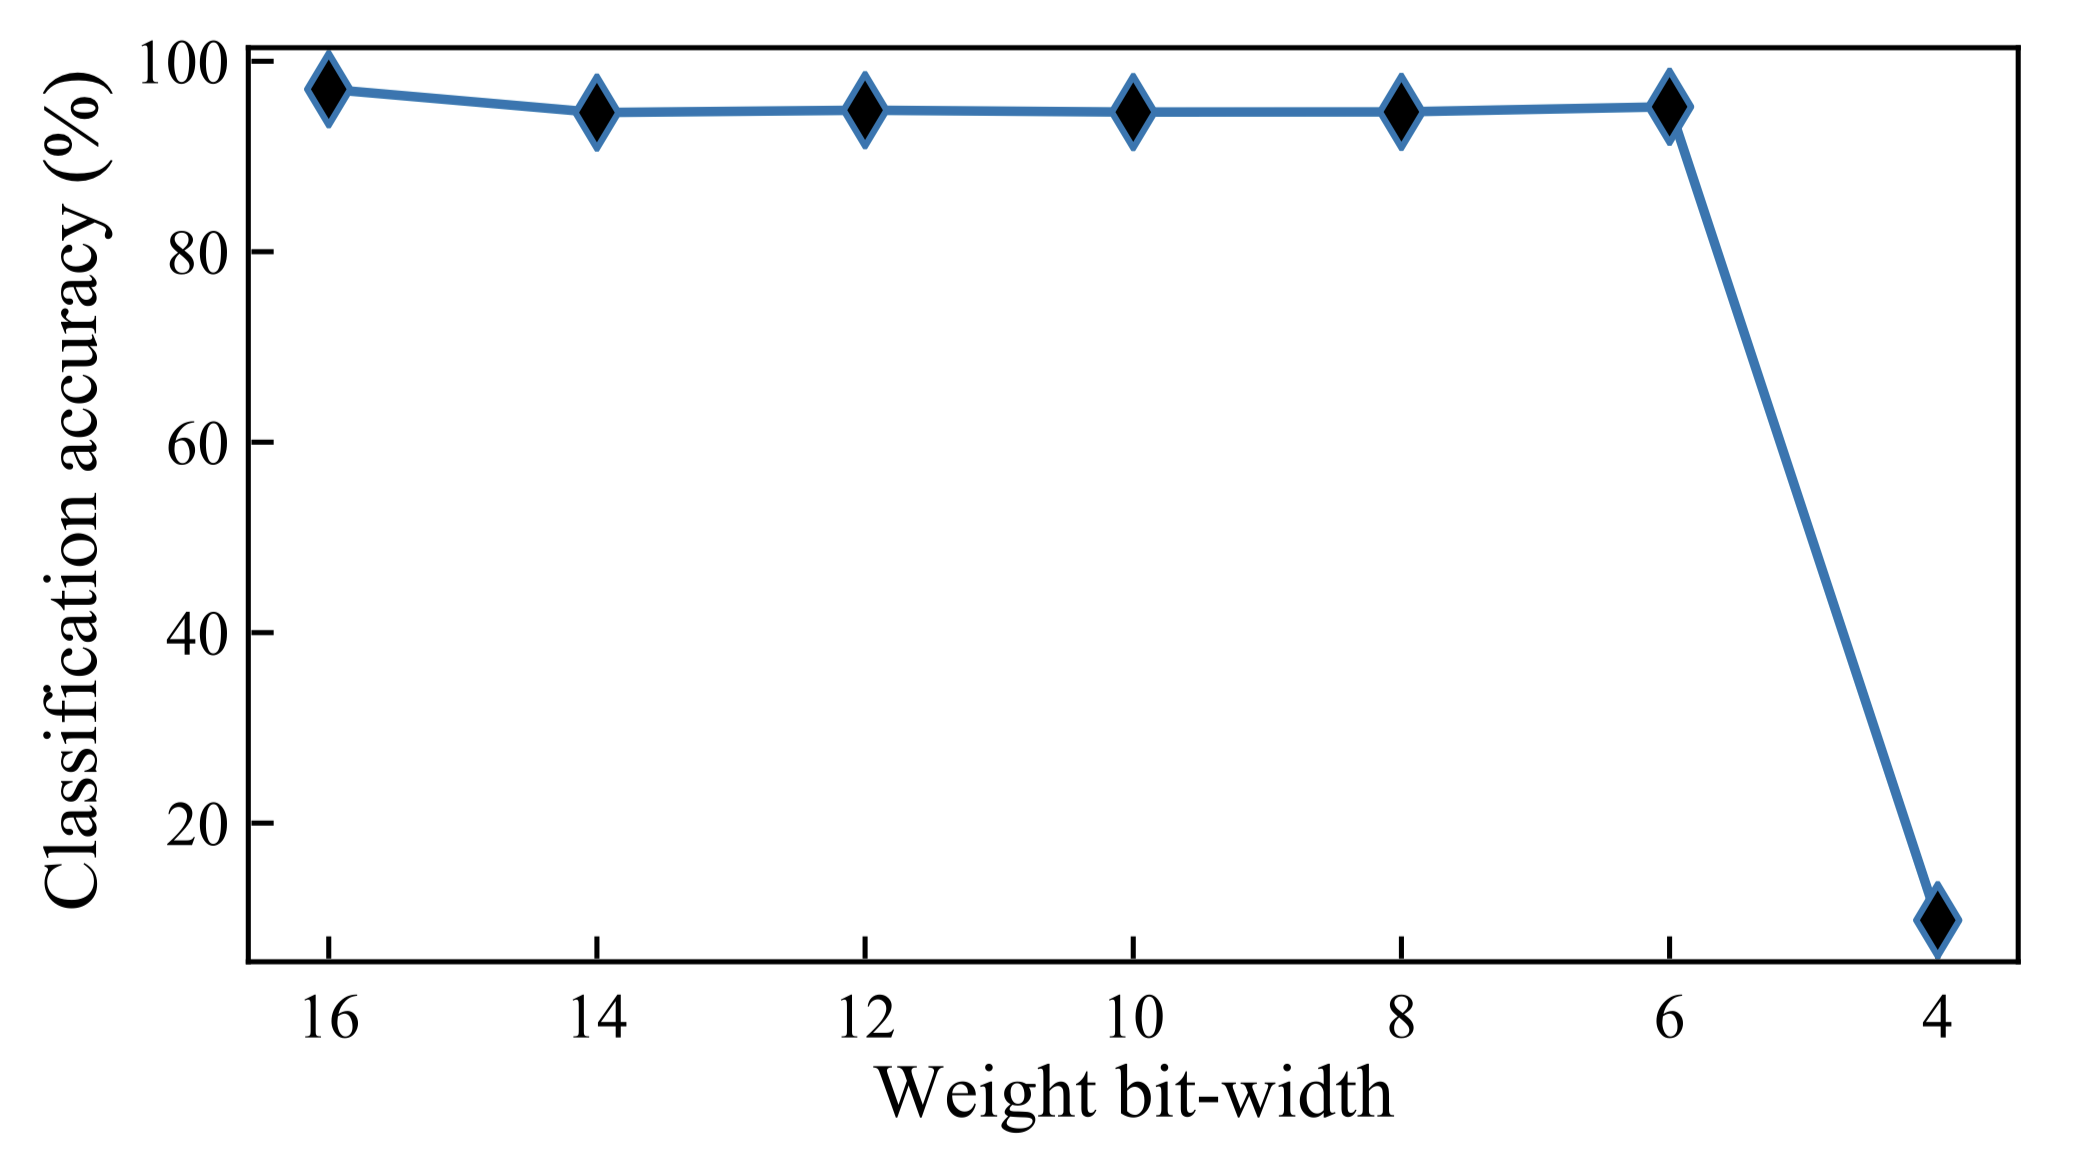
\includegraphics[width=0.8\textwidth]{../assets/Fig5.png}
% \end{center}
% \vspace{-0.1in}  
% \caption{Classification accuracy vs. bit-widths on MNIST.}
% \label{fig:Classification accuracy vs. bit-widths on MNIST.}
% \end{figure}

% \begin{figure}[htb]
% \begin{center}
% 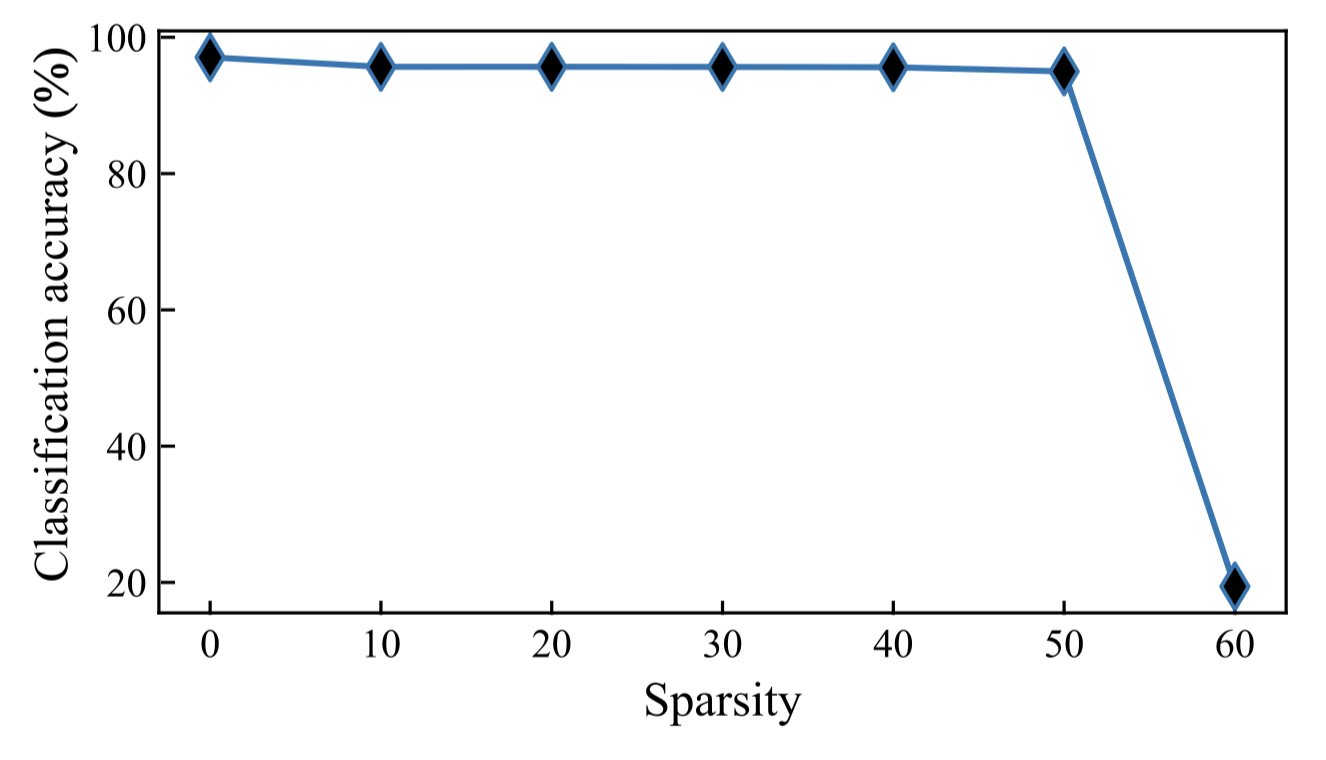
\includegraphics[width=0.8\textwidth]{../assets/Fig6.png}
% \end{center}
% \vspace{-0.1in}  
% \caption{Classification accuracy vs. sparsity on MNIST.}
% \label{fig:Classification accuracy vs. sparsity on MNIST.}
% \end{figure}

% \rule{\linewidth}{0.5pt}

\chapter{讨论}

正如上文第 5 节所述,所提议的 SNN 实现还有进一步优化的机会。 
由于外部存储器带宽对于系统性能至关重要,因此我们在本节中简要讨论降低权重位宽和修剪网络连接的影响。 
我们将这两种技术应用于第 5 节中评估的 MNIST 模型,并使用我们的软件模拟器重新评估分类准确性。

图 5 显示了较低位宽的分类精度。
图 5 所示的结果表明,即使权重位宽降低到 6,位宽对精度的影响也可以忽略不计。
这使得外部数据请求的总大小减少了 62.5\%。 
尽管以如此低的位宽进行操作的能力部分源于 MNIST 数据集的简单性,但减少位宽是提高系统性能的一种有前途的方法。
因此,对于其他系统的实现和基准测试,应仔细考虑位宽的选择。

类似地,网络剪枝的影响如图6所示。
较小值的权重设置为0,并使用稀疏参数作为阈值。
稀疏度为 50\% 时,可以修剪一半的权重,同时分类精度的损失最小。
通过权重修剪,可以减少处理事件所需的权重,从而有利于性能。
我们使用简单的剪枝来掩盖较小的权重; 通过进一步优化,例如微调,可以进一步减少精度损失。

此外,这两种优化技术彼此正交并且可以同时应用。
这需要进一步探索设计空间,留待未来研究。
